%!TEX root = main_arduino_intro.tex

\chapter{Further improvements}\label{chap:outlook}
By now, you have developed a Peltier cooler and can control its set temperature using a few buttons. This project has hopefully also given you a look into how to build scientific setups with Arduino. We elaborated on digital and analog \ac{io} pins in order to control and read all kinds of different sensors and devices. In this last chapter, we will now discuss possible further developments for this project in order to direct the interested reader on what could be done next.


\section{Rigid setup}

The breadboard setup is great for testing and quickly rearranging cables, however, it is not well suited for regular use once you have finished developing your project. If you want to use the developed setup further, several steps can be taken to make it more rigid.

\subsection{Soldering a fixed setup}

To have a more robust setup, it is often worth to solder the components onto a board. One possibility on how to solder the components into place is to use a perma-proto board, see \href{https://www.adafruit.com/product/571}{here} for one example. These boards work similar to the bread board that you used, however, you have to solder all the connections in place. Alternatively, you could use a \href{https://en.wikipedia.org/wiki/Perfboard}{perfboard}, which simply has holes and no lines connected. There are various versions available for these components, and it is ultimately up to you to choose what you prefer.

\begin{figure}[tb]
  \centering
  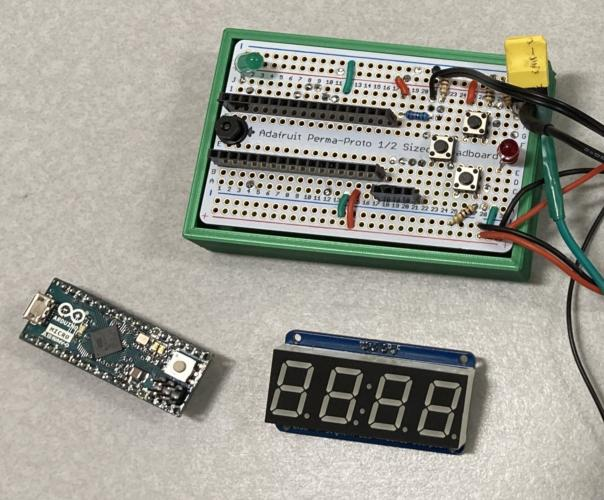
\includegraphics[height=5.5cm]{graphics/06_outlook/final_parts.jpg}
  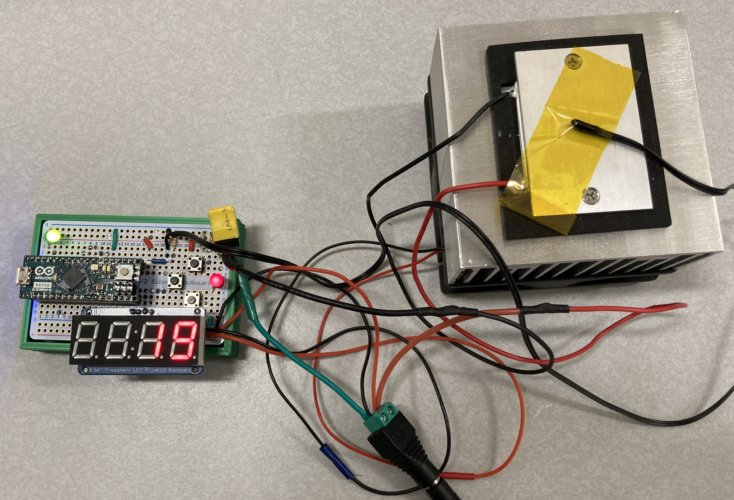
\includegraphics[height=5.5cm]{graphics/06_outlook/final_assembled.jpg}
  \caption{The assembled project with a 3d printed case. Parts unplugged (left) and the assembled project running (right). Most of the cables run underneath the protoboard and are hidden from view.}
  \label{fig:outlook:final_assembled}
\end{figure}
Figure~\ref{fig:outlook:final_assembled} shows an image of the setup that we developed soldered onto an Adafruit perma-proto board. The Arduino and the display in this case are not soldered in place. We rather soldered female headers for these components to plug in. This allows us to easily remove these parts if required.


\subsection{Case}

To have a lab setup that is used actively, it is often useful to not only solder the setup that we want to use regularly, but also to put it in some type of enclosure. Many enclosures are feasible and possible. For example, you could purchase an existing enclosure and simply adopt it for your needs. 

Another possibility is to print an enclosure for your setup using a \href{https://en.wikipedia.org/wiki/3D_printing}{3D printer}. For example, you could design a case using \ac{cad} software such as \href{https://www.freecad.org/}{FreeCAD}. An example for a simple enclosure that keeps the bottom of our setup enclosed is shown in Figure~\ref{fig:outlook:final_assembled}. The FreeCAD and associated files can be found on \href{https://github.com/galactic-forensics/workshop_arduino_electronics/tree/main/3d_files}{GitHub}. Great resources on campus can also be found in the \href{https://www.brandeis.edu/library/research-technology-innovation/makerlab.html}{Brandeis Maker Lab}.


\subsection{\Ac{pcb} development}

Today, there are suppliers that produce small quantities of \acp{pcb} for low prices. It can therefore be worth if your project needs to be duplicated multiple times to design and manufacture a \ac{pcb} for it. Many hints on how to do so can be found online, e.g., \href{https://maker.pro/arduino/projects/7-tips-for-beginners-about-how-to-design-a-pcb-1}{here}. Tools to design \acp{pcb} are, e.g., \href{https://www.kicad.org/}{KiCAD} and \href{https://easyeda.com/}{EasyEDA}. A great resource on campus to consult is the \href{https://www.brandeis.edu/library/research-technology-innovation/automation.html}{Brandeis Automation Lab}.


\section{Proportional control}

When fully assembled, we have seen that our simple implementation was already capable of keeping the Peltier element within 0.5\celsius\ of the set temperature when the thermistor was directly stuck onto the cooling element. This was already achieved when simply turning the controller on and off. However, we have also demonstrated that we can in fact drive the cooler by setting the \ac{pwm} accordingly.

\subsection{\Ac{pid} controller}

A \ac{pid} controller corrects a given system, e.g., our cooler, based on proportional (P), integral (I), and derivative (D) terms. 
\begin{figure}[tb]
  \centering
  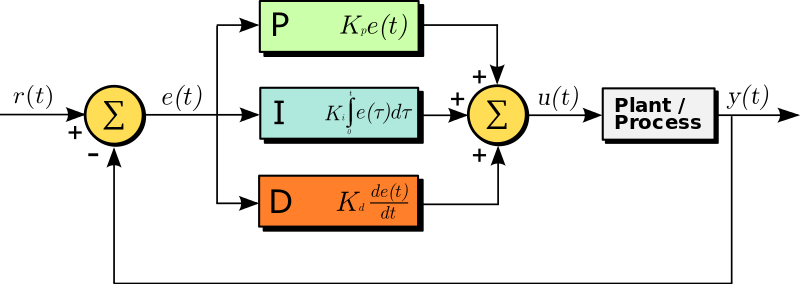
\includegraphics[width=0.8\textwidth]{graphics/06_outlook/pid.png}
  \caption{\ac{pid} control block diagram in a feedback loop. Credit: \href{https://en.wikipedia.org/wiki/File:PID_en.svg}{Arturo Urquizo}, License: \href{https://creativecommons.org/licenses/by-sa/3.0/deed.en}{CC BY-SA 3.0}.}
  \label{fig:outlook:pid}
\end{figure}
Figure~\ref{fig:outlook:pid} shows a block diagram of the control loop for a \ac{pid} controller. The set point is denoted $r(t)$, the achieved point $y(t)$. The ``plant / process'' in this diagram would be our thermoelectric cooler. From the set point and current value, an error $e(t)$ is calculated. Using this error in multiple terms, here all three \ac{pid} terms, a response $u(t)$ is calculated. The overall control function takes the form
\begin{equation}
u(t) = \underbrace{K_p e(t)}_{\equiv P} + \underbrace{K_i \int_0^t e(\tau) d\tau}_{\equiv I} + \underbrace{K_dd \frac{de(t)}{dt}}_{\equiv D}.
\end{equation}
Here, the constants $K_p$, $K_i$, and $K_d$ are positive constants that have to be determined for every system.

In \ac{pid}, the first term (P) will make a proportional response, e.g., if the error $e(t)$ is large, a large correction will be made. The second term (I) integrates all errors that were calculated so far and therefore creates a memory effect. The last term (D) is best described as a prediction value. A much more detailed explanation of \ac{pid} control theory can be found on \href{https://en.wikipedia.org/wiki/PID_controller}{Wikipedia}.


\subsection{Proportional controller for our cooler}

Let us try and implement a proportional feedback for our cooler. Since we can only cool, we can only apply the proportional part when our sample is too warm, otherwise, we will continue to simply turn the Peltier element off and let it warm up by itself. We can apply the proportionality by in- and decreasing the \ac{pwm} output. 

First, let us define $K_p$ in units of K$^{-1}$. At full power, we will drive the \ac{pwm} at 100\%. This level will proportionally drop with lower values of $e(t)$. Since we cannot drive the gate of the \ac{mosfet} with more than 100\%, we will automatically generate a control function that contains a step in it. For a given $K_p$ and a given temperature difference $\Delta T$, we can calculate the response $u(t)$ (from 0 to 1) as:
\begin{equation}
  u(t) = \left\{ 
    \begin{array}{ll}
      K_p \Delta T,   & \Delta T \leq \frac{1}{K_p} \\
      1,              & \Delta T > \frac{1}{K_p}
    \end{array}
  \right.
\end{equation}

An example implementation for $K_p = 2.0\,\mathrm{K}^{-1}$ and our thermoelectric cooler can be found on \href{https://github.com/galactic-forensics/workshop_arduino_electronics/tree/main/further_examples/p_control}{GitHub}. Note that we only had to adopt the \lstinline{void controlTEC()} routine.




\section{Heating and cooling}

The Peltier effect (Section~\ref{sec:tec:peltier_effect}) and thus the thermoelectric cooler can be run in either direction. This means that if we would reverse the polarity of the applied voltage and therefore reverse the current flow, the side that has so far been used as a cooler would start to heat up and the other side would cool down. This also allows us to actively drive the thermoelectric cooler as a heater.

So far, we used one n\ac{mosfet} in order to drive the cooler, see Chapter~\ref{chap:tec}. Adding three more n\acp{mosfet}, we could build a so-called \href{https://en.wikipedia.org/wiki/H-bridge}{H-bridge}. 
\begin{figure}[tb]
    \centering
    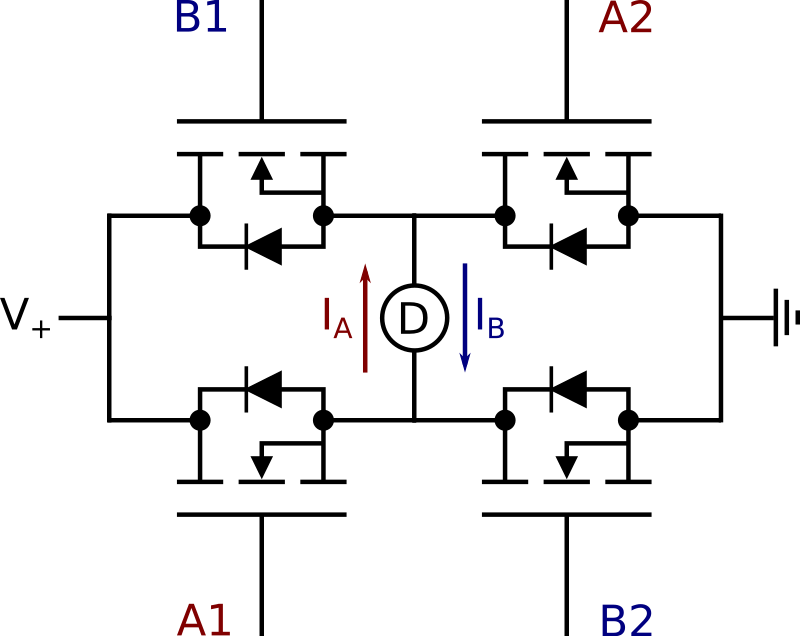
\includegraphics[width=250px]{graphics/06_outlook/h-bridge.png}
    \caption{Schematic of an H-bridge. The ``H'' shape is laying on the side in this Figure. If the \acp{mosfet} labeled A1 and A2 are closed, the current will flow along arrow $I_A$ through device D. If the \acp{mosfet} labeled B1 and B2 are closed, the current will flow along arrow $I_B$. The n\ac{mosfet} drawing is adopted from \href{https://en.wikipedia.org/wiki/Electronic_symbol\#/media/File:Enh_N_channel_Mosfet.svg}{ErikBuer via Wikipedia}, license: \href{https://creativecommons.org/licenses/by-sa/4.0/}{CC BY-SA 4.0}.}
    \label{fig:outlook:h-bridge}
\end{figure}
Figure~\ref{fig:outlook:h-bridge} shows a schematic drawing of an H-bridge. Note that the 
``H'' is laying on its side, the two vertical bars represented by the two n\acp{mosfet} and the horizontal bar with the device D in the middle. If we apply voltage to the gates of the n\acp{mosfet} A1 and A2, the current will flow in direction $I_A$ through the device D. If we, on the other hand, apply voltage to the gates for n\acp{mosfet} B1 and B2, the current flows in the reverse direction, as indicated by arrow $I_B$. 

H-bridges are typically used to drive \ac{dc} motors since the reversal allows us to drive the motor in either direction. You can also find assembled H-bridges online, e.g., \href{https://www.electronics-lab.com/project/5-amp-h-bridge-dc-motor-driver-using-mc33886/}{here}. Make sure that the current rating is appropriate for your application and that you understand how the H-bridge works. For example, the circuit shown in Figure~\ref{fig:outlook:h-bridge} would allow you to short the circuit by opening A1 and B2 or B1 and A2. Such shorts should generally be avoided in order to not damage the components.

\section{Data recording}

\subsection{Record data on storage medium}

Various possibilities exist to log data using an Arduino. For example, you could use a \href{https://www.arrow.com/en/products/1141/adafruit-industries}{data logging shield}, i.e., an extension board, that allows you to plug an SD card into the Arduino and record data on it. Libraries to record data as well as examples can be found on the web, e.g., \href{https://www.arrow.com/en/research-and-events/articles/data-logging-with-arduino-tutorial}{here}.

\subsection{Data in the cloud}

Certain types of Arduino boards that have web capabilities can also be used in combination with the \href{https://docs.arduino.cc/cloud/iot-cloud}{Arduino \ac{iot} cloud}. This allows you to connect your setup to the internet and record measurement points online. A free plan allows you to test out the Arduino \ac{iot} cloud. 

\subsection{Data recording via serial and python}

Another, interesting option is to use the serial interface that Arduino comes with by default and read out the serial commands. Below are example files, full, working examples can be found on \href{https://github.com/galactic-forensics/workshop_arduino_electronics/tree/main/further_examples/data_logger}{GitHub}. 

\paragraph{Arduino setup} We have so far used the serial protocol in order to print information from the Arduino to the serial console. Let us set up an Arduino with an \ac{led} connected to \lstinline{ledPin}. We also store a \lstinline{float result = 23.5}, which is the thing we want to print via serial when asked for it. In the setup, we therefore want to put the following code:
\begin{lstlisting}
void setup() {
  pinMode(ledPin, OUTPUT);
  Serial.begin(9600);
}
\end{lstlisting}
Here, we first set up the \ac{led} as an output, and then initialize the serial interface with a baud rate of 9600 bits per second, see \href{https://www.arduino.cc/en/Serial.Begin}{here} for more information.

Let us assume that we have set up a function called \lstinline{blink_led()} to blink the \ac{led}. We can then set up the main loop code as following:
\begin{lstlisting}
void loop() {

  char inByte;  // where to store the read data
  
  if (Serial.available() > 0) {
    inByte = Serial.read();

    if (inByte == '?') {
      Serial.println(result);
      blink_led();
    } 
  }
}
\end{lstlisting}
Here, we first initialize a variable for one single character. We then ask if Serial data are available and if they are, we read each character into \lstinline{inByte}. It is important. If this character is equal to \lstinline{?}, we print the defined result back to the serial console and blink the \ac{led}, otherwise we do nothing. 

Two things that you should notice here: (1) If you send one question mark from the Arduino serial console, and it is set up to send a newline at the end, you in fact send two characters, a question mark and a newline character. However, the program only responds to the question mark and all other characters are ignored. (2) Note that we send the result using the \lstinline{Serial.println()} command, i.e., we print a newline character at the end of our return. Assuming there are no other newline characters in the result, we can use this line termination scheme to later determine where the result has in fact terminated. This will come in handy further down.


\paragraph{Querying the serial interface with Python}
While the Arduino serial console is great for debugging, it is not made to record and log data on a regular basis. However, we do not need to communicate with the Arduino serial console via the Arduino \ac{ide} but can use any console that can communicate (send and receive commands) via serial in order to build our data logger. Below example shows one very simple way of communicating with the Arduino via the \href{https://www.python.org/}{Python} serial interface. Here, we use the \href{https://pyserial.readthedocs.io/en/latest/pyserial.html}{\texttt{pySerial}}\footnote{The \texttt{pySerial} interface can be installed as: \texttt{pip install pyserial}} library for communication. The following code presents a very simple python script to get and print the result:
\begin{lstlisting}[language=python]
import serial

PORT = "/dev/ttyACM1"

dev = serial.Serial(PORT, 9600)

dev.write(b"?")
result = dev.readline()

print(result)
\end{lstlisting}
We first import the \lstinline{pySerial} package. We then define the \lstinline{PORT} where the Arduino can be found. On a Unix based system, the ports are in the same form as the above example. On Windows however, you would look for something like \lstinline{COM3}. We then assign a variable \lstinline{dev} to the device and use the \lstinline{pySerial} package to open communication with the serial port. To query the temperature, we have to send a question mark to the Arduino. We can do so using the \lstinline{write} command and send a question mark that has been encoded to binary, i.e., \lstinline{b"?"}. We then read the next line that came back from the device, store it as a \lstinline{result}, and then print this stored value. Note that the \lstinline[language=python]{dev.readline()} command works only if you send a newline command from the Arduino, e.g., by using \lstinline{Serial.println()}.

Once you run this program, which can be found \href{https://github.com/galactic-forensics/workshop_arduino_electronics/blob/main/further_examples/data_logger/simple_query.py}{here on GitHub}, you will see that (1) the \ac{led} blinks when the program runs and (2) that the string \lstinline{b'23.50\r\n'} is returned. The returned string is of course also binary encoded and, in order to get a regular string as you are used to, you would have to decode this binary string. Furthermore, you might want to strip the carriage return (\lstinline{\r}) and newline (\lstinline{\n}) characters at the end of the line. You could clean up the result string as following:
\begin{lstlisting}[language=python]
result = float(result.decode("utf-8").rstrip())
\end{lstlisting}
This decodes the result, strips the empty characters on the right side of the string, and then converts it to a float. 

We can of course also extend this simplest possible example into an actual data logger. A simple example how this could be achieved in Python can be found on GitHub with the filename \href{https://github.com/galactic-forensics/workshop_arduino_electronics/blob/main/further_examples/data_logger/data_logger.py}{\lstinline{data_logger.py}}. The python file is extensively commented and records a given set of measurements with defined intervals in between and saves them as a \ac{csv} file. The important part to remember is the following: The serial interface allows you to easily control and drive the Arduino from your computer. If you adjust your firmware accordingly, you will be able to interact with your Arduino by other means than just the Arduino \ac{ide}, e.g., via Python. This can be extremely useful for further development and data recording.